\documentclass{beamer}
\usetheme[usetitleprogressbar,nosmallcapitals]{m}
\usepackage{wasysym}
\usepackage{amsmath}
\usepackage{minted}

\usepackage{filecontents}

\newenvironment{slide}[1]
	{\begin{frame}[fragile,environment=slide]{#1}}
	{\end{frame}}

\newcommand {\fullimage}[1] {
	\begin{center}
		\includegraphics[width=\textwidth,height=0.8\textheight,keepaspectratio]{#1}
	\end{center}
}

\newcommand\blfootnote[1]{%
	\begingroup
	\renewcommand\thefootnote{}\footnote{#1}%
	\addtocounter{footnote}{-1}%
	\endgroup
}

\title{Neuro Computer Architektur}
\subtitle{Innovative Rechnerarchitekturen}
\date{21. Januar 2016}
\author{Johannes Elsmann, Max Taube}
\institute{HTWK Leipzig}

\begin{document}
\maketitle


\begin{slide}{Ablauf}
	\tableofcontents
\end{slide}

\section{Künstliche neuronale Netze}

\begin{slide}{Künstliche neuronale Netze}
	\begin{itemize}
		\item Zweig der künstlichen Intelligenz
		\item Nach biologischem Vorbild
		\item Netz aus "Neuronen"
		\item Liefert Ausgabewert zu Eingaben
		\item Kann von Beispielen Lernen
	\end{itemize}
	\begin{center}
		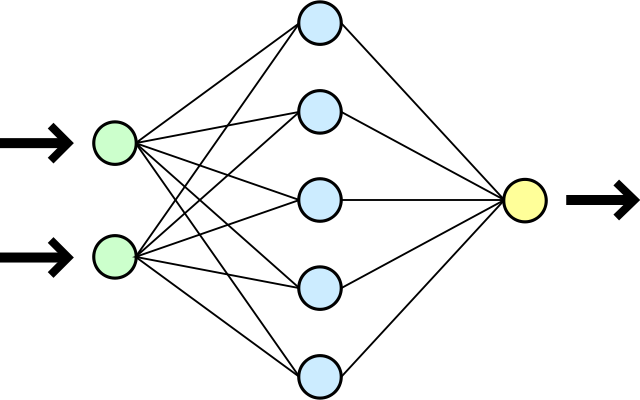
\includegraphics[width=\textwidth,height=0.4\textheight,keepaspectratio]{content/Neural_network}
	\end{center}
\end{slide}

\begin{slide}{Neuron}
	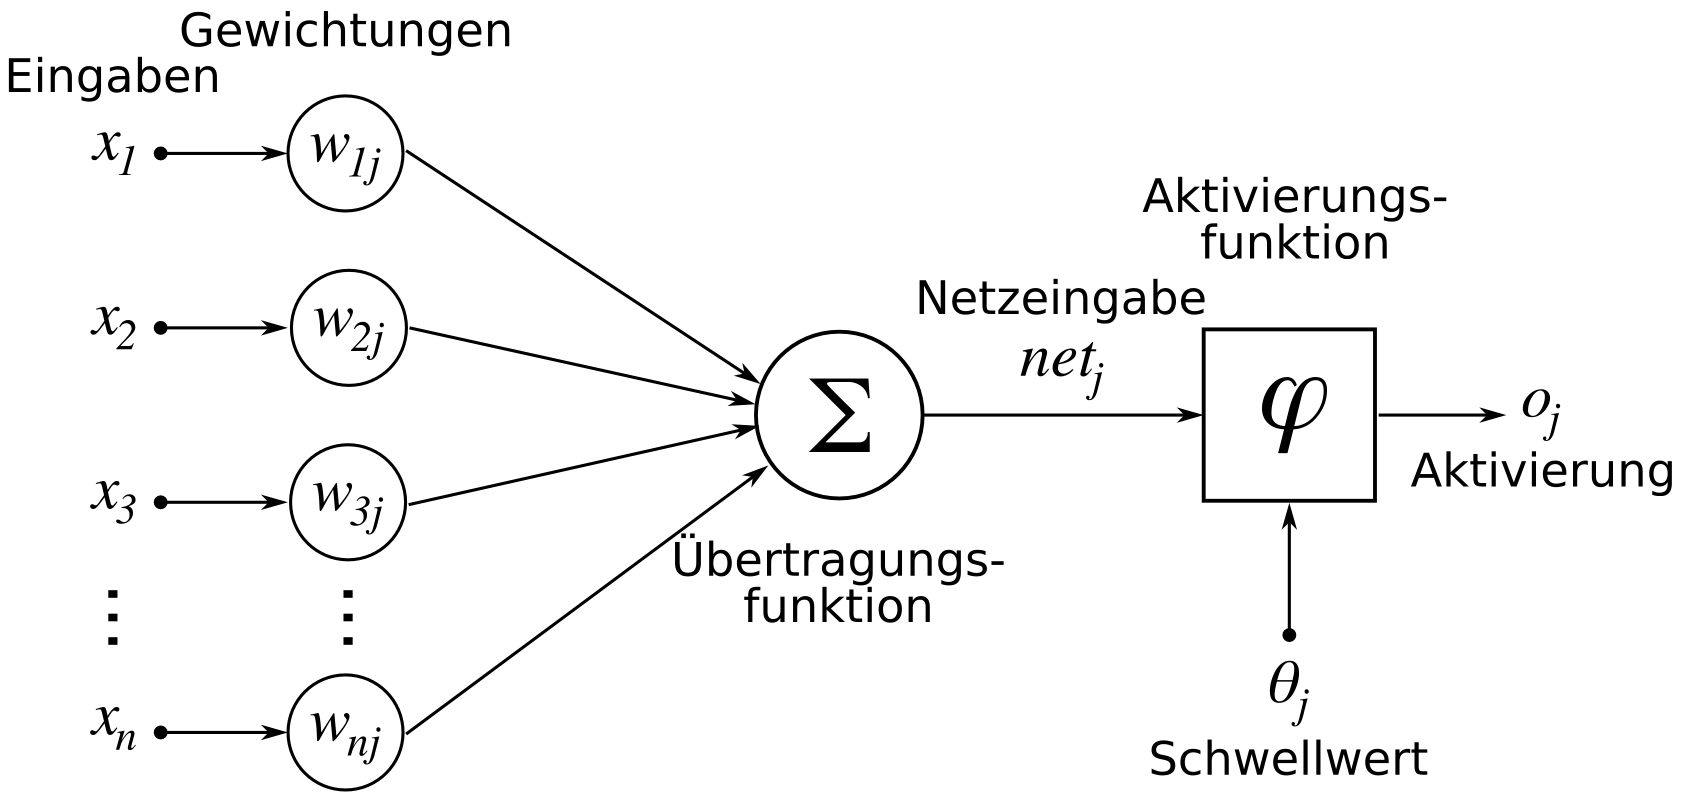
\includegraphics[width=\textwidth,height=0.8\textheight,keepaspectratio]{content/ArtificialNeuronModel}
	\blfootnote{„ArtificialNeuronModel deutsch“ von Chrislb. Lizenziert unter CC BY-SA 3.0 über Wikimedia Commons}
\end{slide}

\begin{slide}{Netzwerk}
	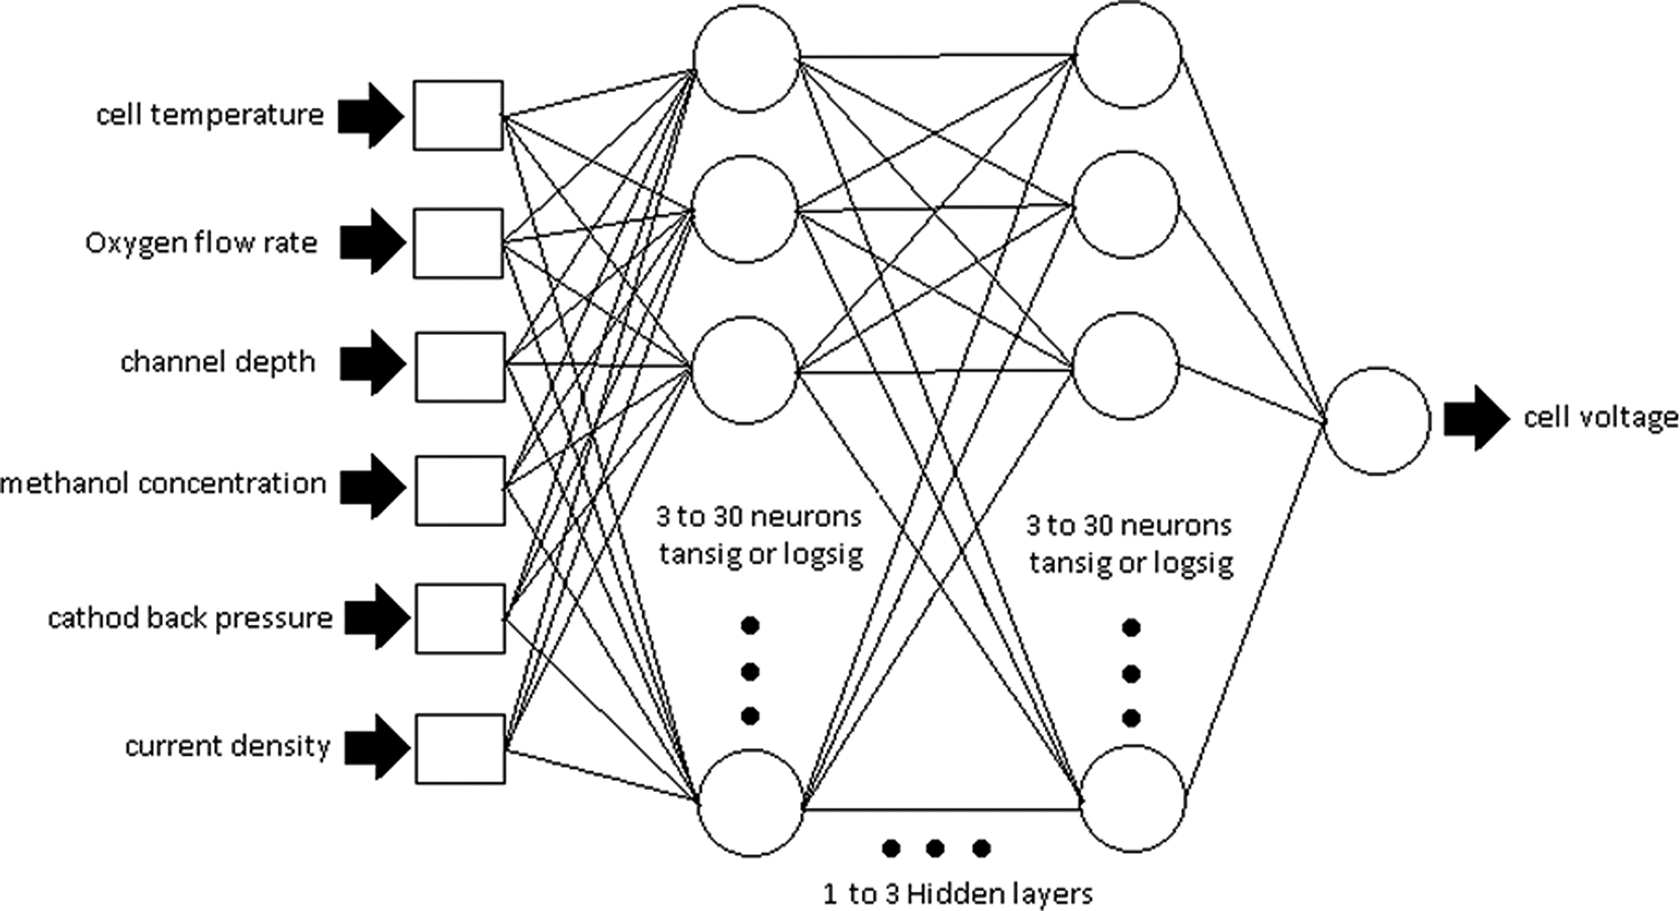
\includegraphics[width=\textwidth,height=0.8\textheight,keepaspectratio]{content/knn_fuel}
	\blfootnote{Tafazoli M, Baseri H, Alizadeh E, Shakeri M. Modeling of Direct Methanol Fuel Cell Using the Artificial Neural Network. ASME. J. Fuel Cell Sci. Technol. 2013}
\end{slide}

\begin{slide}{Künstliche neuronale Netze}
	\begin{itemize}
		\item lernen durch anpassen von Gewichten
		\item verschiedene Lernalgorithmen
		\item anlernen von Eingabe-Ausgabe-Paaren
	\end{itemize}
\end{slide}


\begin{slide}{Anwendung}
	Besonders geeignet wenn wenig systematisch nutzbares Wissen vorliegt.
	\begin{itemize}
		\item Texterkennung
		\item Bilderkennung
		\item Gesichtserkennung
		\item Prognosen
		\item Frühwarnsysteme
		\item KI in Spielen und Simulationen
	\end{itemize}
\end{slide}

\section{Motiv}

\begin{slide}{Von Neumann Stärken}
	Stärken der von Neumann Architektur sind
	\begin{itemize}
		\item Universeller Einsatz
		\item Synchrone / Getaktete Verarbeitung
		\item Logik / Algorithmik
		\item Geschwindigkeit
	\end{itemize}
\end{slide}

\begin{slide}{Von Neumann Schwächen}
	Die von Neumann Architektur zeigt in bestimmten Einsatzgebieten schlechte Performanz.
	
	Schwierige Einsatzgebiete bei zeitkritischer Betrachtung sind bspw.
	\begin{itemize}
		\item Verarbeitung hochdimensionaler (verrauschter) Daten
		\item Gesichts- und Spracherkennung / Allg. Mustererkennung
		\item Sensoren-Netzwerke
	\end{itemize}
	
	Für die Verarbeitung in \alert{Echtzeit} ist je nach Anwendungsgebiet zum Teil ein sehr hoher Energieaufwand nötig.
\end{slide}

\begin{slide}{Motiv KNN Nutzung}
	Der Einsatz von \textbf{Künstlich Neuronalen Netzen} ist in den vorgestellten Problemgebieten zum Teil sehr erfolgreich. Ihre Simulation unter der von Neumann Architektur verhindert jedoch teilweise theoretische Vorteile.
\end{slide}

\begin{slide}{Motiv Neuro Architektur}
	Durch Entwicklung einer geeigneten Architektur für KNN erhofft man sich
	
	\begin{itemize}
		\item Hoch skalierbare Netzwerke
		\item Massive Parallelität
		\item Sehr geringen Energieaufwand
		\item Fehlertoleranz
		\item Geschwindigkeit
	\end{itemize}
	
	Vorbild dafür sind die Fähigkeiten des menschlichen Gehirns bei gerade einmal 20W Energieverbrauch.
\end{slide}

\begin{slide}{Profitierende Anwendungsgebiete}
	Von der Entwicklung von Neuro Chips profitieren vor allem zeitkritische Anwendungsgebiete, die bereits jetzt (theoretisch) von KNN profitieren.
	
	\begin{itemize}
		\item Autonomes Fahren
		\item Echtzeit Video Analyse
		\item Sensoren Netzwerke
	\end{itemize}
\end{slide}
\section{Architekturen}

\begin{slide}{Architekturen}
	\begin{itemize}
		\item Bla
	\end{itemize}
\end{slide}


\section{Ausblick}

\begin{slide}{Ausblick}
	\begin{itemize}
		\item Bla
	\end{itemize}
\end{slide}


\begin{frame}{Quellen}
  \raggedright
  \nocite{*}
  \bibliographystyle{plain}
  {\scriptsize \bibliography{literature}}
\end{frame}

\end{document}